\documentclass[final]{fhnwreport}         %[mode] = draft or final
%%---Main Packages-----------------------------------------------------------------------
\usepackage[english, ngerman]{babel}	%Mul­tilin­gual sup­port for LaTeX
\usepackage[T1]{fontenc}				      %Stan­dard pack­age for se­lect­ing font en­cod­ings
\usepackage[utf8]{inputenc}				  %Ac­cept dif­fer­ent in­put en­cod­ings
\usepackage{lmodern}                 %The newer Font-Set
\usepackage{textcomp}					      %LaTeX sup­port for the Text Com­pan­ion fonts
\usepackage{graphicx} 					      %En­hanced sup­port for graph­ics
\usepackage{float}						        %Im­proved in­ter­face for float­ing ob­jects
%\usepackage{ifdraft}                %Let you check if the doc is in draft mode

%%---Useful Packages---------------------------------------------------------------------
\usepackage[pdftex,dvipsnames]{xcolor}  %Driver-in­de­pen­dent color ex­ten­sions for LaTeX
\usepackage{csquotes}                   %Simpler quoting with \enquote{}
\usepackage{siunitx} 					     %A com­pre­hen­sive (SI) units pack­age
\usepackage{listings}					     %Type­set source code list­ings us­ing LaTeX
\usepackage[bottom]{footmisc}			  %A range of foot­note op­tions
\usepackage{footnote}					     %Im­prove on LaTeX's foot­note han­dling
\usepackage{verbatim}					     %Reim­ple­men­ta­tion of and ex­ten­sions to LaTeX ver­ba­tim
\usepackage[textsize=footnotesize]{todonotes} %Mark­ing things to do in a LaTeX doc­u­ment
\usepackage{lipsum}              % Gives you access to blindtext
\usepackage[acronym]{glossaries}
\makeglossaries 
\usepackage{pgfgantt}
\hypersetup{colorlinks=true, urlcolor=blue}

%%---Tikz Packages-----------------------------------------------------------------------
%\usepackage{standalone}
%\usepackage{tikz}
%\usepackage{circuitikz}
%\usetikzlibrary{arrows}
%\usetikzlibrary{calc}
%\usetikzlibrary{intersections}

%%---Math Packages-----------------------------------------------------------------------
\usepackage{amsmath}					    %AMS math­e­mat­i­cal fa­cil­i­ties for LaTeX
%\usepackage{amssymb}					  %Type­set­ting symbols (AMS style)
%\usepackage{array}						  %Ex­tend­ing the ar­ray and tab­u­lar en­vi­ron­ments
%\usepackage{amsthm}					    %Type­set­ting the­o­rems (AMS style)

%%---Table Packages----------------------------------------------------------------------
\usepackage{tabularx}					  %Tab­u­lars with ad­justable-width columns
%\usepackage{longtable}
\usepackage{multirow}					  %Create tab­u­lar cells span­ning mul­ti­ple rows
\usepackage{multicol}					  %In­ter­mix sin­gle and mul­ti­ple columns

%%---PDF / Figure Packages---------------------------------------------------------------
\usepackage{pdfpages}					  %In­clude PDF doc­u­ments in LaTeX
\usepackage{pdflscape}					  %Make land­scape pages dis­play as land­scape
%\usepackage{subfig}					    %Fig­ures di­vided into sub­fig­ures

%%---Other Packages----------------------------------------------------------------------
%\usepackage{xargs}              %De­fine com­mands with many op­tional ar­gu­ments


%%---Main Settings-----------------------------------------------------------------------
\graphicspath{{./graphics/}}			%Defines the graphicspath
%\geometry{twoside=false}				%twoside=false disables the "bookstyle"
\setlength{\marginparwidth}{2cm}
\overfullrule=5em						    %Creates a black rule if text goes over the margins => debugging

%%---User Definitions--------------------------------------------------------------------
%%Tabel-Definitions: (requires \usepackage{tabularx})
\newcolumntype{L}[1]{>{\raggedright\arraybackslash}p{#1}}    %column-width and alignment
\newcolumntype{C}[1]{>{\centering\arraybackslash}p{#1}}
\newcolumntype{R}[1]{>{\raggedleft\arraybackslash}p{#1}}					                        %loads all packages, definitions and settings	

%%%%% Logo: Hocvhschule HTU oder HSI, Sprache DE oder EN:
%\newcommand{\logofilename}{FHNW_HTU_DE}
%\newcommand{\logofilename}{FHNW_HTU_EN}
\newcommand{\logofilename}{FHNW_HSI_DE}
%\newcommand{\logofilename}{FHNW_HSI_EN}
%%%%%
%%%%% Bibliographie entweder im IEEE- oder im APA-Stil:
%\usepackage[style=ieee,urldate=comp,backend=biber]{biblatex}
\usepackage[style=apa,urldate=comp,backend=biber]{biblatex}
%%%%%
\addbibresource{literature/bib.bib}
											
\title{Cloud Governance in einer multi-provider Cloud}  %Project Title
\author{Projektvereinbarung IP5}    %Document Type => Technical Report, ...
\date{Windisch, März 2025}               %Place and Date

\begin{document}

\pagenumbering{roman}	

%%---TITLEPAGE---------------------------------------------------------------------------
\selectlanguage{ngerman}                  %ngerman or english
\maketitle

\vfill

\begin{figure}[H]
\centering
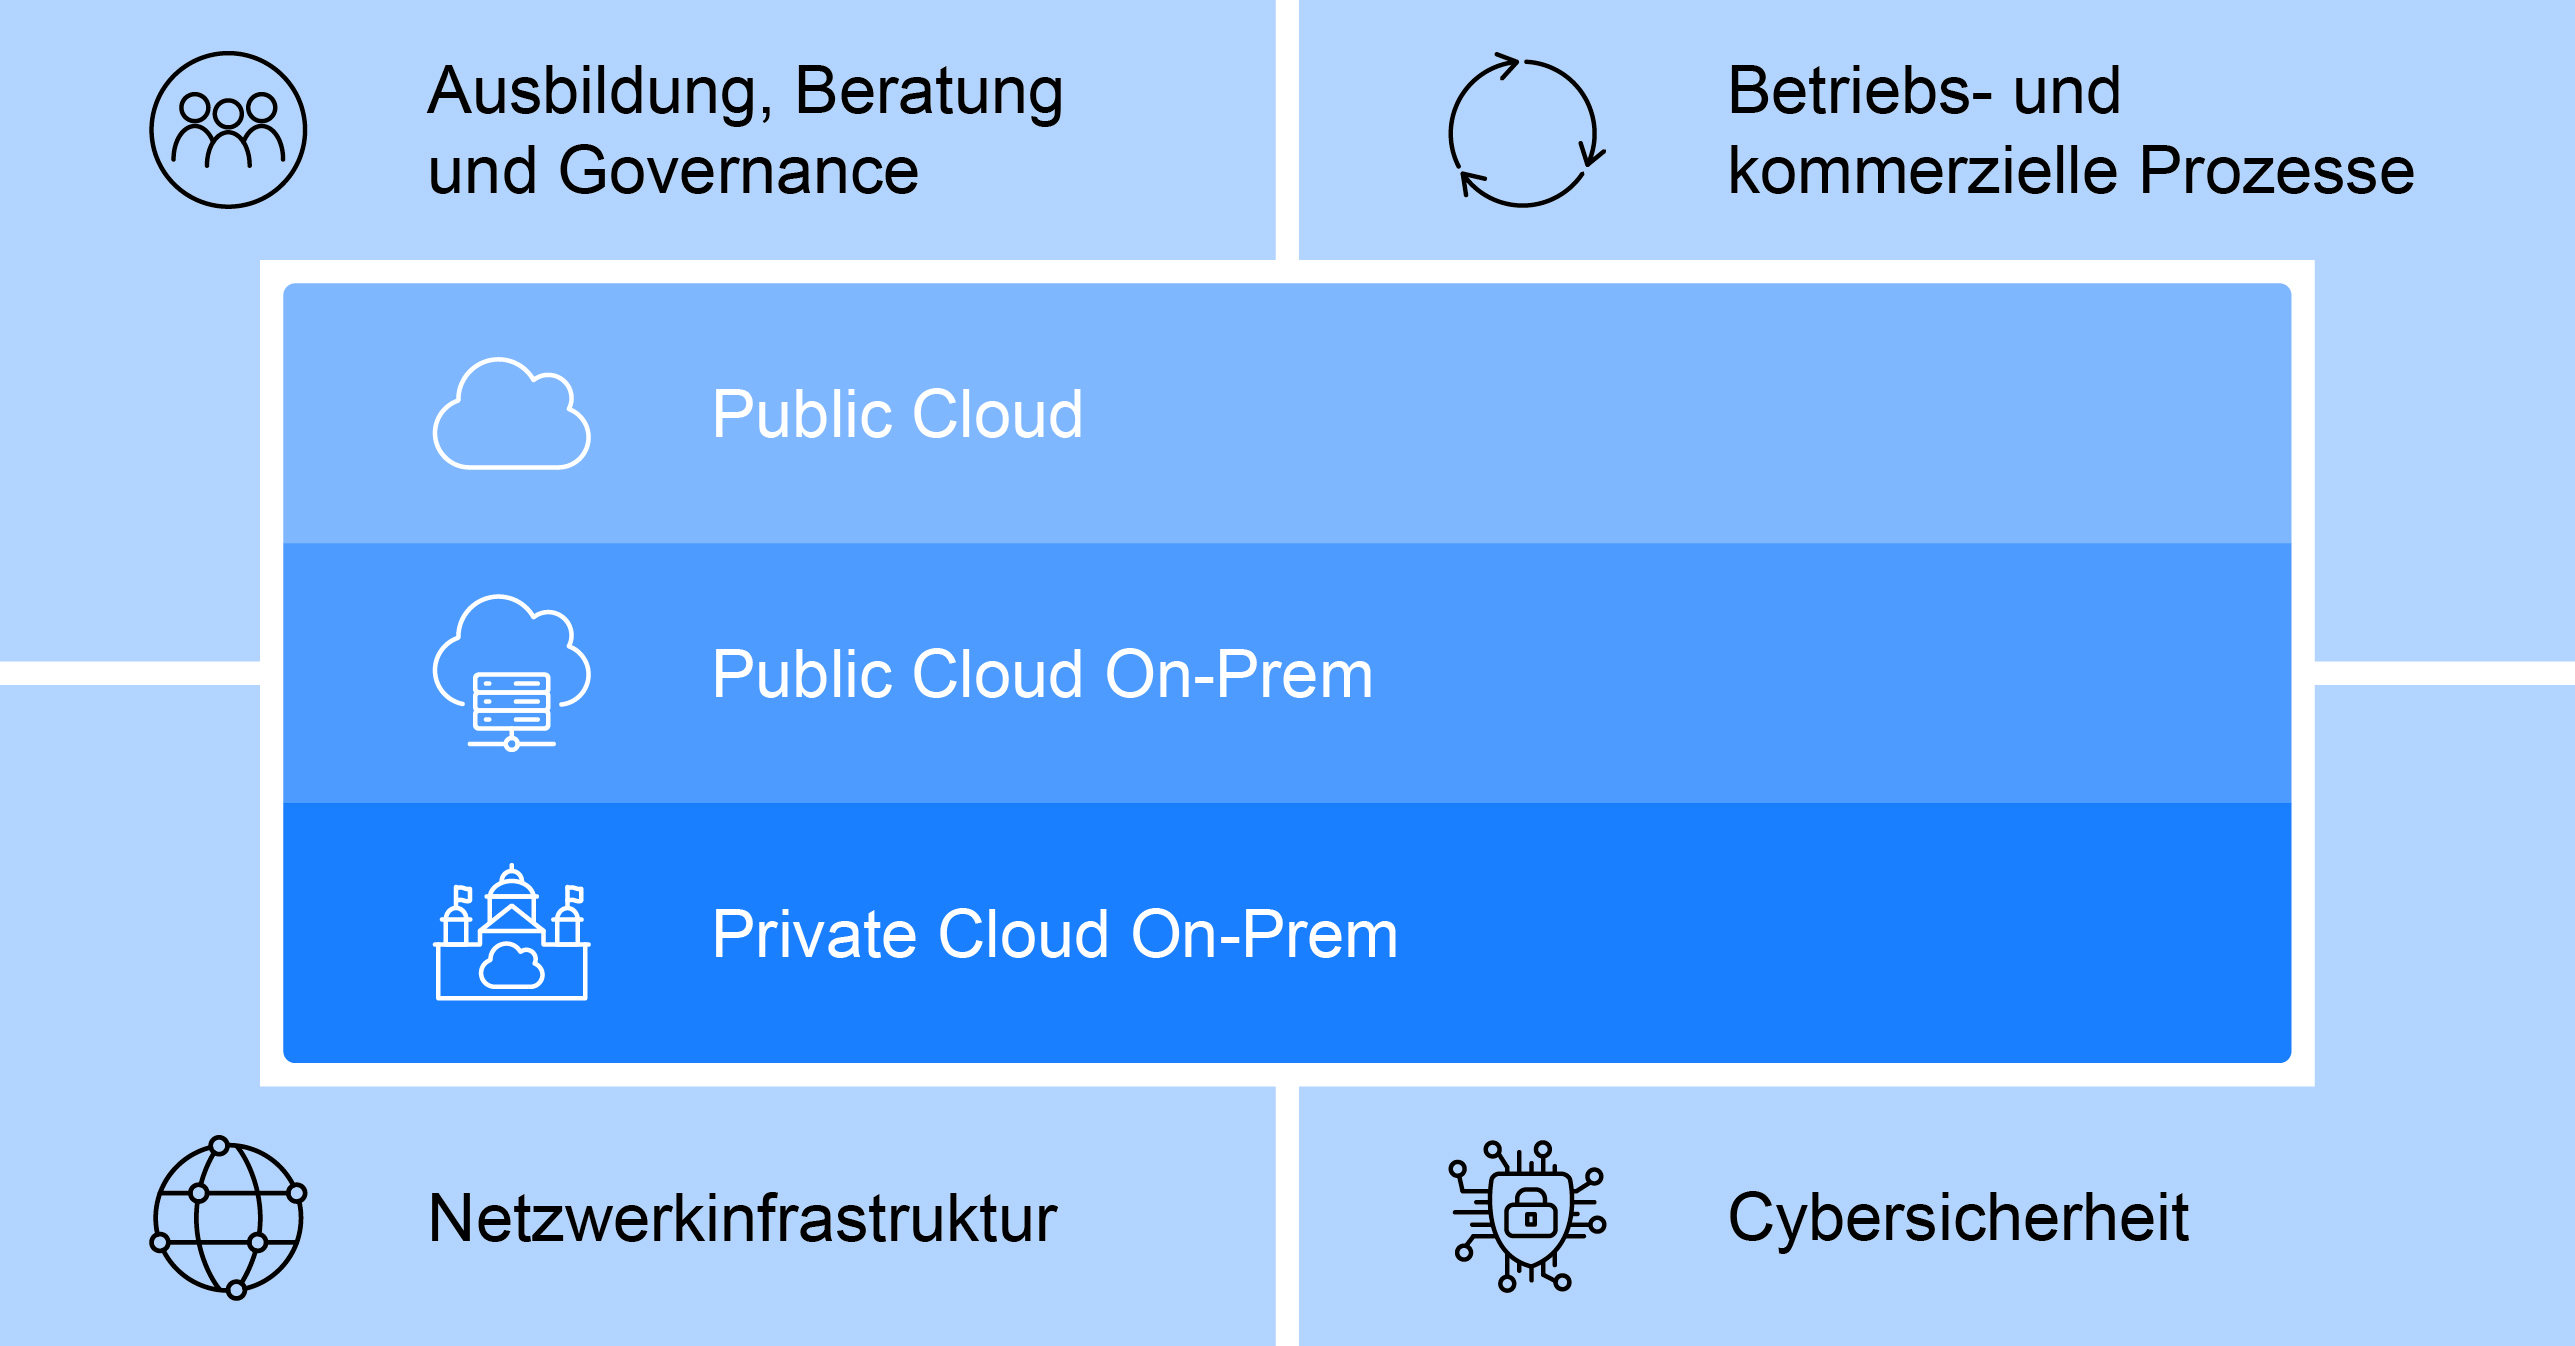
\includegraphics[width=\linewidth]{BIT_SGC_Overview.jpg}
\end{figure}

\vfill

\begin{tabular}{@{}p{5cm} l}
  Studentin/Student          &    Frithjof Hoppe\\
  &    Benjamin Dätwyler\\[2ex]
Expertin/Experte           &    Sebastian Matyas\\[2ex]
Fachbetreuer/in            &    Sebastian Graf\\[2ex]
Auftraggeberin             &    Thierry Perroud\\[2ex]
Projektnummer              &    25FS\_IMVS29\\[4ex]
\multicolumn{2}{@{}l}{Fachhochschule Nordwestschweiz, Hochschule für Informatik}
\end{tabular}

\vspace*{4ex}
% Logo Industriepartner
\begin{tikzpicture}[remember picture,overlay,every node/.style={anchor=north east}]
  \node at (current page.north east) [xshift=-1cm, yshift=-1cm] {
\includegraphics[width=8cm]{BIT_d_rgb_pos_quer_pf.jpg}};
\end{tikzpicture}

\clearpage
			
%%---ABSTRACT----------------------------------------------------------------------------
\selectlanguage{ngerman}				%ngerman or english
\thispagestyle{empty}

%%---TABLE OF CONTENTS-------------------------------------------------------------------	
\selectlanguage{ngerman}				%ngerman or english
\tableofcontents
\clearpage

% \listoffigures
% \listoftables
% \cleardoublepage

%%---TEXT--------------------------------------------------------------------------------
\pagenumbering{arabic}
\section{Ausgangslage}

Das Bundesamt für Informatik und Telekommunikation verfolgt mit dem Swiss Government Cloud (SGC) Vorhaben die Transformation der Cloud-Infrastruktur der Bundesverwaltung. Vision ist es einen auf die Bedürfnisse des Bundes zugeschnittene hybride Multi-Cloud Infrastruktur aufzubauen.

\begin{figure}[H]
    \begin{center}
        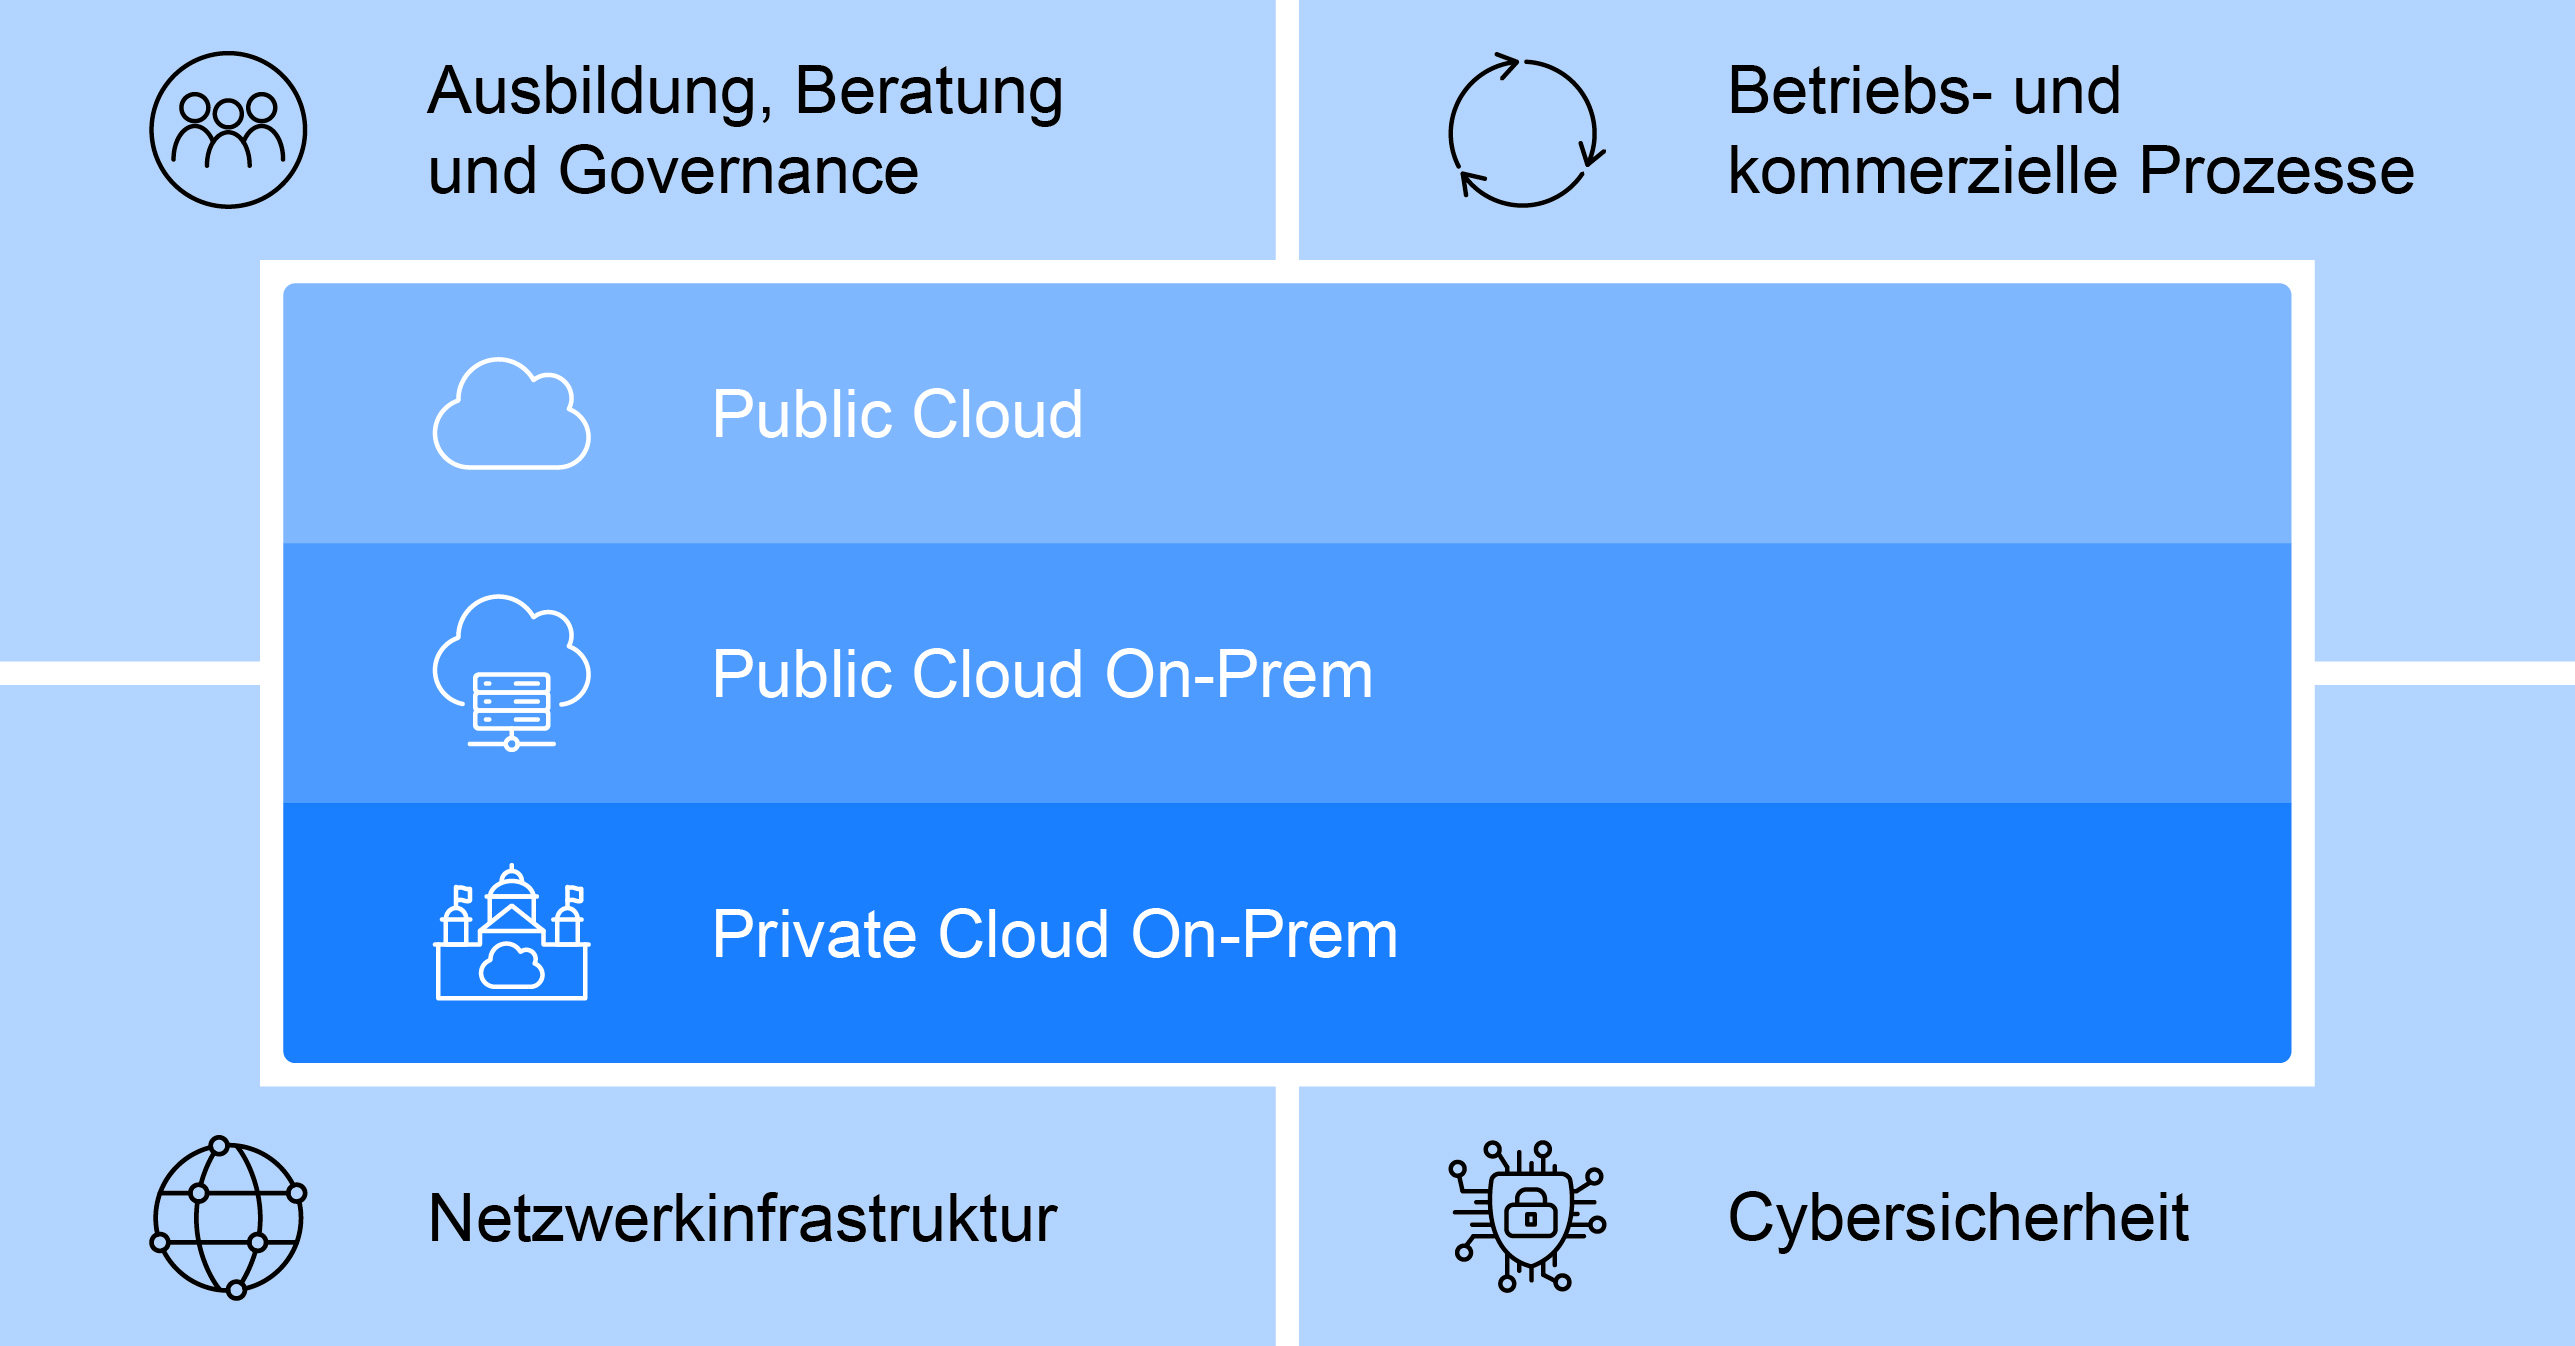
\includegraphics[width=\linewidth]{BIT_SGC_Overview.jpg}
    \end{center}
\caption{Das Vorhaben SGC im Überblick}
\label{fig:sgc_overview}
\end{figure}

Heute verteilt sich die Infrastruktur des Bundesamt für Informatik und Telekommunikation (nachfolgenden als BIT bezeichnet) vereinfacht dargestellt wie folgt:

\begin{itemize}
\item OnPremise/Private-Cloud Hosting Umgebung welches durch das BIT selbst betrieben wird
\item Public-Cloud Hosting Umgebung bei unterschiedlichen Cloud-Anbietern wie Microsoft Azure und Amazon AWS
\end{itemize}

\section{Problemstellung}

Mit dem Betreiben von Services geht die Einhaltung von governance Regeln einher.

Die Sicherheitsanforderungen der Fachanwendungen entstehen oft aus Standards / Richtlinien / Normen der BV welche manuell und plattformspezifisch umgesetzt werden.
Nennenswert ist hier u.A. Si001 für den IT Grundschutz in der Bundesverwaltung welcher ein Mindestmass an Vorgaben gibt.

Die daraus resultierenden Regeln werden oft unterschiedlich definiert, abgelegt und angewendet.
Zusätzlich besteht die Gefahr, dass Standards/Richtlinien/Normen der BV unterschiedlich interpretiert werden können und somit dann andere Regeln angewendet werden.

Mit Ausblick auf das SGC Vorhaben bekommt diese Situation nochmals mehr an Bedeutung weil die Anzahl an Plattformen steigt und es somit schwieriger wird die Übersicht zu wahren.
\section{Zielsetzung}

\subsection{Forschungsfragen}

% TODO Si001 anhängen

\subsubsection{Compliance-Aspekte}

\textit{Welche wichtigen Aspekte eines Schutzobjektes sind für die Compliance zu berücksichtigen?}

// Frage aus meeting mit Graf am 05.03. ZU löschen? \textit{Welche wichtigen Aspekte sind für die Compliance auf der SGC zu berücksichtigen?
Wie können diese Aspekte auf die verschiedenen Plattformen angewendet werden? Wie werden diese Aspekte heute innerhalb des BITs implementiert?}


Die einzelnen Serviceangebote der Cloud-Provider bieten jeweils unterschiedliche Servicelevel, zum Teil auch variierend zwischen Standorten. Die wichtigsten Aspekte (von Schutzobjekten) welche in eine Complianceprüfung gehören sollen identifiziert werden.

Wir wollen erforschen, wie ein Mapping zwischen den relevanten Eigenschaften von Services in der Cloud und den Aspekten von Schutzobjekten implementiert werden kann.

% Verfügbarkeit, Skalierbarkeit, Sicherheit, CIA-> alles was so compliance sein könnte

\subsubsection{Erforschung bestehende Produkte, Konzepte, Ansätze und Frameworks}

\textit{Welche Konzepte und etwaige Produkte existieren bereits zur plattformübergreifenden Prüfung und Enforcement von Compliance?}

Im Rahmen der Lösungsfindung soll von bereits bestehenden Produkten profitiert werden. Wir wollen herausfinden, welche Produkte bereits existieren und wie diese die Complianceprüfung durchführen.
Nützliche Ansätze und Konzepte sollen hervorgehoben und für eine allfällige Eigenimplementation ggf. in Betracht gezogen werden. Hier wollen wir Produkte untersuchen welche die Complianceprüfung direkt/proprietär umsetzen, unabhängig von der dahinterliegenden Technologie.

\textit{Welche bestehenden Frameworks, Sprachen oder Konzepte sind am besten geeignet zur Umsetzung von cloud-übergreifender Compliance?}

Schutzobjekte (z.B. Applikationen) werden in der SGC cloud-nativ (via zugehörigem Deployment Code) deployed. Somit wäre der Deployment Code der richtige Ort festzulegen, welche Compliance-Regeln eingehalten werden müssen. Wir möchten hier Konzepte, Ansätze und Frameworks erforschen, welche die cloud-native Umsetzung der Compliance ermöglichen.

% Abgrenzung zu SIEM

\subsubsection{Konzeption eines Frameworks}

\textit{Wie muss ein Framework Compliance Regeln implementieren sodass eine Anwendung durch verschiedenen Interessengruppen möglich ist?}

Um verschiedenen Regelwerke (Si001 etc.) einheitlich anzuwenden ist eine Art Sprache notwendig die es den verschiedenen Experten (sei es CISO, Projektverantwortlichen) erlaubt ihre Bedürfnisse auszuformulieren. Diese muss gleichzeitig durch ein System interpretiert werden können damit die entsprechenden Massnahmen ergriffen werden können.

\subsection{Ziele}
Die folgenden Ziele gelten für die gesamte Arbeit und orientieren sich an den Forschungsfragen. Aktuell wird davon ausgegnagen dass die Erkenntinsse in einem Artefakt resultieren welches die genantne Ziele implementiert. Dieses Artefakt wird nachfolgend als Framework bezeichnet welches jedoch die Art umd des Artefakts nicht einschränken soll.

\begin{table}[H]
    \centering
    \begin{tabularx}{\textwidth}{|l|X|}
        \hline
        \textbf{\#} & \textbf{Ziel} \\
        \hline
        1 & Ein Konzept für die technische Umsetzung einer plattformübergreifenden (mindestens zwei Public on eine Private Cloud) Cloud-Governance im Rahmen des SGC-Vorhabens bis zum 14.08.2025 umgesetzt \\
        \hline
        2 & Ein Framework welches mindestens die Ist-Situation einer multi plattformübergreifende Cloud-Umgebung gegenüber Governancen Vorgaben analysiert ist bis zum 14.08.2025 umgesetzt  \\
        \hline
    \end{tabularx}
    \caption{Ziele}
    \label{tab:goals}
\end{table}

\subsubsection{Abgrenzung}

Bei der Thematik die behandelt werden soll handelt es sich um ein weites Feld, weshalb die Zielerreichung wie folgt eingeschränkt wird:

\begin{itemize}
    \item Das Framework deckt einen Servicetyp (z.B. k8s) einer Public-Cloud Plattform ab
    \item Das Framework deckt einen Servicetyp einer Public-Cloud und einer private Cloud Plattform des BIT ab
    \item Das Framework deckt mindestens zwei Public-Cloud Plattformen und eine private Cloud Plattform ab
    \item Das Framework kann mindestens reaktiv zur Prüfung der Compliance eingesetzt werden
\end{itemize}

\subsection{Meilensteine}

Die folgenden Meilensteine sind ebenfalls im 

\begin{table}[H]
    \centering
    \begin{tabularx}{\textwidth}{|l|l|X|}
        \hline
        \textbf{\#} & \textbf{Datum} & \textbf{Meilenstein} \\
        \hline
        1 & 09.03.2025 & Projektvereinbarung signiert
        \\
        \hline
        2 & xx.xx.xx & Bestehenden Praktiken der verschiedenen internen Interessen-
        gruppen sind bekannt
        % TODO Anforderungen im sinne von wie die bestehenden policies ausgelegt / interpretiert werden \newline
        % TODO Produkte bspw CSPM, CIEM, CWPP
        \\
        \hline
        2 & xx.xx.xx & Recherche von bestehenden Produkten, deren Funktionalität, Gemeinsamkeiten und Deckung von Anforderungen ist erfolgt
        % TODO Anforderungen im sinne von wie die bestehenden policies ausgelegt / interpretiert werden \newline
        % TODO Produkte bspw CSPM, CIEM, CWPP
        \\
        \hline
        3 & xx.xx.xx & erster Entwurf Konzept für Framework
        \\
        \hline
        3 & xx.xx.xx & Implementation erster PoC
        \\
        \hline
        3 & 14.08.25 & Abgabe Arbeit
        \\
        \hline
    \end{tabularx}
    \caption{Meilensteine}
    \label{tab:milestones}
\end{table}
\section{Technologien}
 
Die effektiv verwendeten Technologie ergeben sich erst durch die Arbeit.
Folgende Liste soll einen ungefähren Eindruck ergeben, die Motivation aufzeigen und ist nicht abschliessend:

\begin{itemize}
    \item \textbf{Infrastructure as Code und Policy as Code} IaC Tool wie Terraform oder Pollumi provisionieren von Ressourcen in Cloud-Umgebugen. Ähnlich dazu besitzten die verschiedenen Cloud-Provider ihre eigenen Configuration Languages und services. Diese können als Basis für eine eigenen DSL dienen. Beispiele: Azure Sentinel, Open Policy Agent / Rego
    \item \textbf{Public Cloud / Hyperscaler} Repräsentiert durch die verschiedenen grösseren Plattformen wie AWS, Azure, (RedHat) Openshift im potentiellen SGC Umfeld dienen diese uns als Analyse-Objekte
    \item \textbf{CSPM Tools} Cloud services posture management richet unterstützt unter Anderem die Erkennung und Abwehr von Risiken in Bezug auf eine Cloud-Umgebung und die allg Einhaltung von Vorgaben. Hier exisieren von diversen Hyperscalern bereits Plattformen von denen wir profitieren können. Beispiele: Azure Defender, AWS Security Hub etc.
    \item  \textbf{CWPP Tools} Cloud workfload protection tools erkennen die workload welche in einer bspw Cloud-Umgebung vorhanden sind und führt automatisch Bewertungen durch. Tools bzw die Idee dieser Art könnten die Grundlage für unser angedachtes Framework darstellen. Beispiele: Falco, Twistlock
    \item \textbf{}
\end{itemize}
\section{Projektorganisation}

Das ip5 Projekt läuft ab der Freigabe der Projektvereinbarung bis zum 14.08.2025. Die erbrachte Leistung sollte den erwarteten 180h pro Teammitglied entsprechen.
Wir orientieren uns hierzu an der agilen Methodik Kanban. Hierunter verstehen wir konkret, dass:
\begin{itemize}
    \item Die verschiedenen Tasks werden für jeden Projektbeteiligten sichtbar geführt (TODO hier link GithubBoard)
    \item Das Team inklusive dem PO synchen sich mindestens alle zwei Wochen um den aktuellen Stand zu tracken
    \item Die Arbeit erfolgt nicht in sprints sondern allg nach Priorität welche aus den jeweiligen Syncs hervorgeht
    \item Den Stakeholde wird alle 4 Wochen der aktuelle Stand präsentiert, bei welchem sie Ihren Input eingeben können
\end{itemize}

\subsection{Austausch}
Der Austausch inklusive den Synch wird zwischen den beteiligten erfolgt bevorzugt über den vorgesehen \href{https://teams.microsoft.com/l/channel/19%3A3bd20805200e482b809e5bf7b9294922%40thread.tacv2/25FS%20SGCWorkloadClassification?groupId=5c45c1ea-5d01-4a7b-8989-82ab37a27223&tenantId=9d1a5fc8-321e-4101-ae63-530730711ac2&ngc=true}{Teams-Kanal}, damit alle Interessierten auch passiv teilnehmen können.

\begin{table}[H]
    \centering
    \begin{tabularx}{\textwidth}{|l|X|}
        \hline
        \textbf{Objekt} & \textbf{Ort} \\
        \hline
        Projektarbeit & Die Projekt arbeit wird auf \href{https://gitlab.fhnw.ch/cloudgovernance/ip5-paper}{im ip5-paper repo} als LaTex Dokument abgelelgt \\
        \hline
        % TODO korrekten Link abglegen
        Code-Basis & Die verschiedenen Code-Bases werden unter ein separaten \href{TODO-link}{Github Organization} im Sinne des EMBAG öffentlich abgelegt  \\
        \hline
    \end{tabularx}
    \caption{Verwendete Plattformen}
    \label{tab:used-plattforms}
\end{table}


\begin{landscape}
\subsection{Zeitplan}
Das folgende Gantt-Diaramm stellt die Arbeit mit den Meilensteinen und groben Tasks da. Zu erwähnen ist hierbei, dass die detaillierten Tasks mittels Kanban-Board getracked werden.


\newcounter{myWeekNum}
\stepcounter{myWeekNum}
%
\newcommand{\myWeek}{\themyWeekNum
    \stepcounter{myWeekNum}
    \ifnum\themyWeekNum=53
         \setcounter{myWeekNum}{1}
    \else\fi
}
%
%%% Begin document
\setcounter{myWeekNum}{8}
\ganttset{%
calendar week text={\myWeek{}}%
}
%
\begin{figure}[h!bt]
\begin{center}
\begin{ganttchart}[
vgrid={*{6}{draw=none}, dotted},
x unit=.1cm,
y unit title=.6cm,
y unit chart=.6cm,
time slot format=isodate,
time slot format/start date=2025-02-17]{2025-02-17}{2025-08-18}
    \ganttset{bar height=.6}
    \gantttitlecalendar{year, month=name, week} \\
    
    % Kickoff
    \ganttgroup{Kickoff}{2025-02-17}{2025-03-07} \\
        \ganttbar{Austausch Kunde}{2025-02-17}{2025-02-28} \\
        \ganttmilestone[milestone/.append style={fill=red}]{Proj Vereinbarung signiert}{2025-02-28} \\

    % Analyse
    \ganttgroup{Analyse}{2025-03-03}{2025-03-14} \\
        \ganttbar{Interessengruppen}{2025-03-03}{2025-03-14} \\
        \ganttbar{Literatur und Recherche}{2025-03-03}{2025-03-14} \\
        \ganttmilestone[milestone/.append style={fill=red}]{Analyse dokumentiert}{2025-03-14} \\
    
    
    % Konzeptionierung / Implementierung
    \ganttgroup{Konzeptionierung}{2025-03-17}{2025-04-18} \\
        \ganttbar{Definieren DSL}{2025-03-17}{2025-04-04} \\
        \ganttbar{Erprobung DSL}{2025-04-07}{2025-04-11} \\
        \ganttmilestone[milestone/.append style={fill=red}]{First draft DSL}{2025-04-18} \\
    
    
    % CODE FREEZE
    \ganttmilestone[milestone/.append style={fill=red}]{Code freeze}{2025-07-14} \\


    \ganttgroup{Dokumentieren}{2025-07-14}{2025-08-18} \\


    \ganttbar[bar/.append style={fill=brown}]{Projektwoche}{2025-05-05}{2025-05-10} \\
    \end{ganttchart}
    \end{center}
    \caption{Time Plan}
\end{figure}
\end{landscape}

%%---BIBLIOGRAPHY------------------------------------------------------------------------
% {\sloppypar
% \printbibliography[heading=bibintoc, title=Quellenverzeichnis]
% }

\newacronym{CSB}{CSB}{Cloud Service Broker}
\newacronym{CAPS}{CAPS}{Cloud Application Plattform Services}

%%---APPENDIX----------------------------------------------------------------------------
% \section*{Eigenständigkeitserklärung}
\markboth{\MakeUppercase{Eigenständigkeitserklärung}}{\MakeUppercase{Eigenständigkeitserklärung}}

\addcontentsline{toc}{section}{Eigenständigkeitserklärung}

Ich (wir) erkläre(n) hiermit, dass ich (wir) den vorliegenden Leistungsnachweis selber und selbständig verfasst habe(n),
\begin{itemize} 
\item dass ich (wir) sämtliche nicht von mir (uns) selber stammenden Textstellen und anderen Quellen wie Bilder etc. gemäss gängigen wissenschaftlichen Zitierregeln\footnote{z.B. APA oder IEEE} korrekt zitiert und die verwendeten Quellen klar sichtbar ausgewiesen habe(n); 
\item dass ich (wir) in einer Fussnote oder einem Hilfsmittelverzeichnis alle verwendeten Hilfsmittel (KI-Assistenzsysteme wie Chatbots\footnote{z.B. ChatGPT}, Übersetzungs-\footnote{z.B. Deepl} Paraphrasier-\footnote{z.B. Quillbot} oder Programmierapplikationen\footnote{z.B. Github Copilot}) deklariert und ihre Verwendung bei den entsprechenden Textstellen angegeben habe(n);
\item dass ich (wir) sämtliche immateriellen Rechte an von mir (uns) allfällig verwendeten Materialien wie Bilder oder Grafiken erworben habe(n) oder dass diese Materialien von mir (uns) selbst erstellt wurde(n);
\item dass das Thema, die Arbeit oder Teile davon nicht bei einem Leistungsnachweis eines anderen Moduls verwendet wurden, sofern dies nicht ausdrücklich mit der Dozentin oder dem Dozenten im Voraus vereinbart wurde und in der Arbeit ausgewiesen wird; 
\item dass ich mir (wir uns) bewusst bin (sind), dass meine (unsere) Arbeit auf Plagiate und auf Drittautorschaft menschlichen oder technischen Ursprungs (Künstliche Intelligenz) überprüft werden kann;
\item dass ich mir (wir uns) bewusst bin (sind), dass die Hochschule für Technik FHNW einen Verstoss gegen diese Eigenständigkeitserklärung bzw. die ihr zugrundeliegenden Studierendenpflichten der Studien- und Prüfungsordnung der Hochschule für Technik verfolgt und dass daraus disziplinarische Folgen (Verweis oder Ausschluss aus dem Studiengang) resultieren können.
\end{itemize}

\vspace*{4ex}

Windisch, tt. Monat 20jj

\vspace*{4ex}

{\renewcommand{\arraystretch}{2}
\begin{tabular}{@{}>{\bf}ll}
Name: & Pia Musterfrau\\
Unterschrift: & \\[6ex]
Name: & Michael Mustermann\\
Unterschrift: & \\
\end{tabular}
% \selectlanguage{english}				%ngerman or english
% \section*{Declaration of Authenticity}
\markboth{\MakeUppercase{Declaration of Authenticity}}{\MakeUppercase{Declaration of Authenticity}}

\addcontentsline{toc}{section}{Declaration of Authenticity}

I hereby declare that any individual work / pair work / team work submitted for assessment is entirely the product of my own / my own and my partner’s / my own and my team’s effort,
\begin{itemize} 
\item that I/we have correctly cited all text passages that do not originate from me/us, in accordance with standard academic citation rules\footnote{e.g. APA oder IEEE}, and that I/we have clearly mentioned all sources used; 
\item that I/we have declared in footnotes or in an index of auxiliary tools all aids used (AI assistance systems such as chatbots\footnote{e.g., ChatGPT}, translation\footnote{e.g., DeepL}, paraphrasing\footnote{e.g., Quillbot}, or programming applications\footnote{e.g., Github Copilot}, and indicated their use at the corresponding text passages;
\item that I/we have acquired all intangible rights to any materials I/we may have used, such as images or graphics, or that these materials were created by me/us; 
\item that the topic, the thesis or parts of it have not been used in an assessment of another module, unless this has been expressly agreed with the lecturer in advance and is stated as such;
\item that I/we am/are aware that my/our work may be checked for plagiarism and for third-party authorship of human or technical origin (artificial intelligence); 
\item that I/we am/are aware that the FHNW School of Engineering will pursue a violation of this declaration of authenticity and that disciplinary consequences (reprimand or expulsion from the study program) may result from this.
\end{itemize}

\vspace*{4ex}

Windisch, tt. Monat 20jj

\vspace*{4ex}

{\renewcommand{\arraystretch}{2}
\begin{tabular}{@{}>{\bf}ll}
Name: & Pia Musterfrau\\
Signature: & \\[6ex]
Name: & Michael Mustermann\\
Signature: & \\
\end{tabular}
% \selectlanguage{ngerman}				%ngerman or english
\printglossary[type=acronym, title=Abkürzungsverzeichnis]  %
\begin{appendix} %Anhang
\section{Si001}

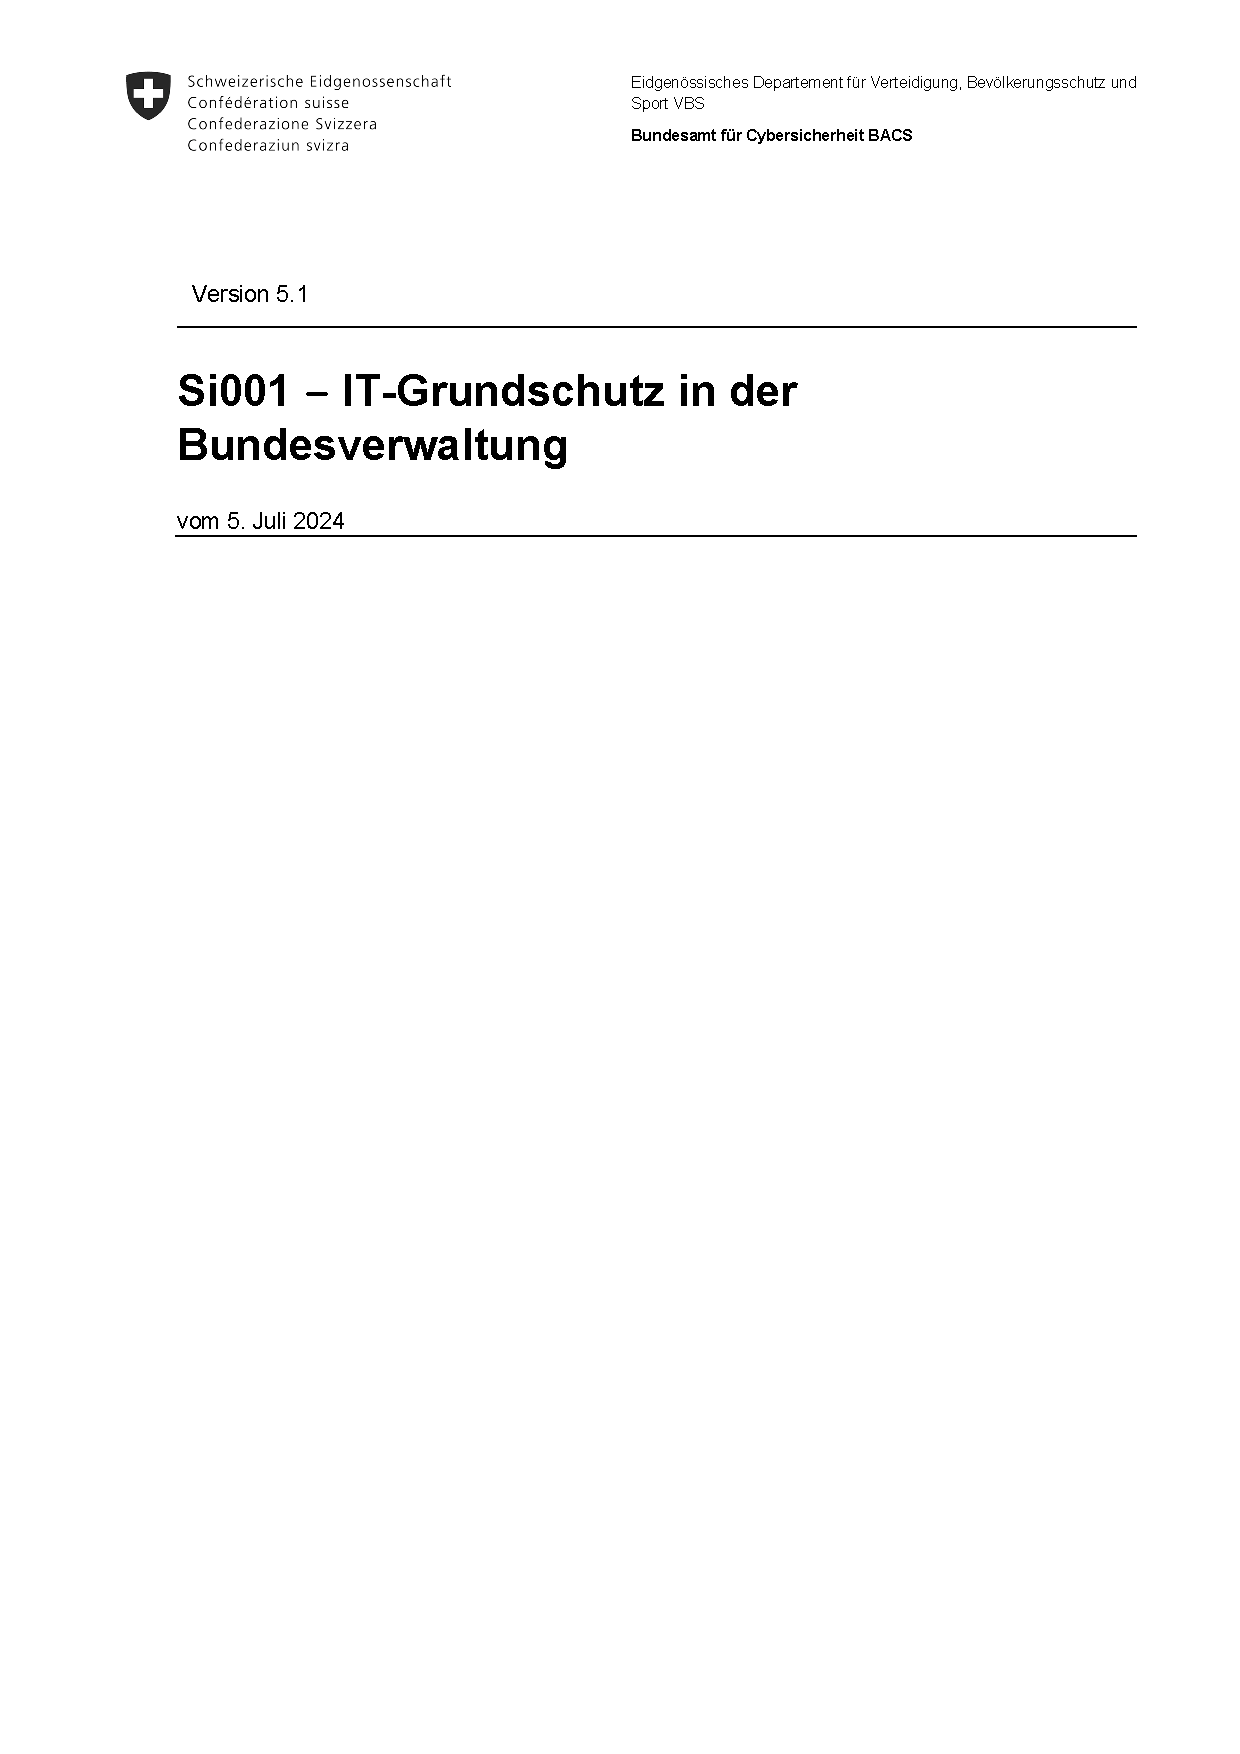
\includepdf[pages={1-27}]{appendix/Si001-IT-Grundschutz_V5-1-d.pdf}

\end{appendix}


%%---NOTES for DEBUG---------------------------------------------------------------------
%\newpage
%\listoftodos[\section{Todo-Notes}]
%\clearpage

\end{document}